% The document class marks this as a poster, supplying various options that
% control rendering of some standard features (e.g., the title bar).

\documentclass[ % the name of the author
                    author={Liam O'Shea},
                % the name of the supervisor (preferably including title)
                supervisor={Dr. Sion Hanunna},
                % the thesis    title (which cannot be blank)
                     title={ZeroToHero},
                % the thesis subtitle (which can    be blank)
                  subtitle={},
                % the degree programme (from BSc, MEng, MSci, MSc and PhD)
                    degree={Bsc},
                % the year of submission
                      year={2014} ]{poster}

\usepackage{epstopdf}
\usepackage{algorithm2e}
\begin{document}

% -----------------------------------------------------------------------------

\begin{frame}{} 

\vfill

\begin{columns}[t]
    \begin{column}{0.900\linewidth}
    \begin{block}{\normalsize Introduction}
    \small Computer aided coaching has revolutionised training approaches and been a key driver
            in improving sports performance at the highest level. Professional athletes can now use
            advanced augmented coaching to accurately and reliably measure a range of metrics that
            are then used as indicators of performance. ZeroToHero implements punch classification \& qualitative assessment of boxing pose and technique using the Kinect, a low cost consumer device that can bring specialist boxing coaching to everyone.{\newline}
            This research is borne out of a desire to improve access and cost to boxing coaching which are problems I have encountered first hand through the University Boxing Club. In the wider environment It could be used in developing countries where physical access to coaches with the
            required expertise may be difficult as well as local clubs in the UK.

    \end{block}
    \end{column}
\end{columns}

\vfill

\begin{columns}[t]
    \begin{column}{0.422\linewidth}
    \begin{block}{\normalsize 1. Kinect Data}
    \small The Kinect Skeleton API is used to get data from 20 joints
    \begin{figure}[h]
        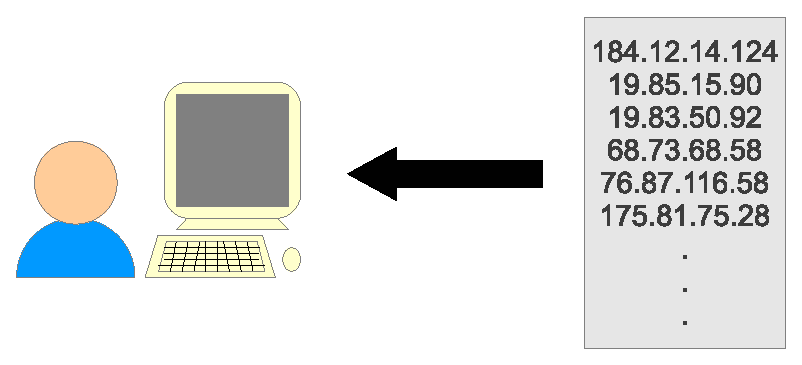
\includegraphics{diagrams/poster_get_list.eps}
    \end{figure}
    The sender then sends messages to the receiver by sending packets with a spoofed source IP address to every IP address in the shout list.
    \begin{figure}[h]
        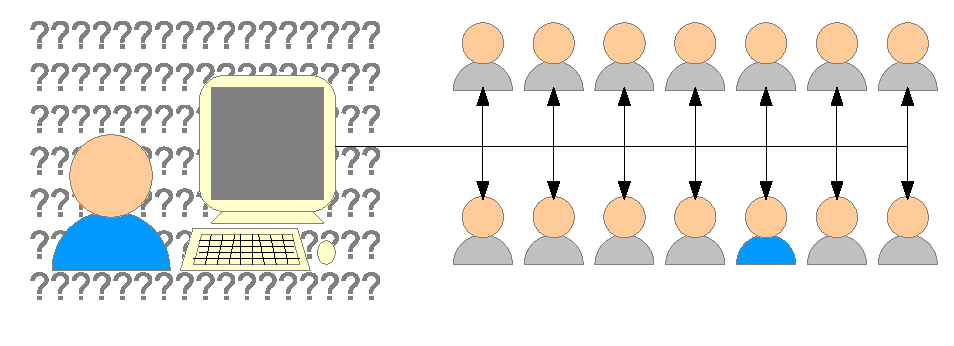
\includegraphics{diagrams/poster_d2.eps}
    \end{figure}
    This method of communication is unreliable and very inefficient but it does remove most of the information about the peers' identities. The point of most concern is that some party could search through the IP addresses in the shout list to find the true identity of the peer. For this reason, shout groups have been created.
    \end{block}
    \end{column}

    \begin{column}{0.422\linewidth}
    \begin{block}{\normalsize 2. Punch Segmentation}
    \small Sets of data were recorded from local boxers, university boxers and professional boxers to `ground-truth' my data. Dimensionality reduction was performed on raw skeleton data before using a set of heuristic rules to find the beginning of each punch.
    Evenly spaced samples are taken from each punch and used as a set of features for that type of punch.

    % \begin{figure}[h]
    % \begin{flushright}
    %     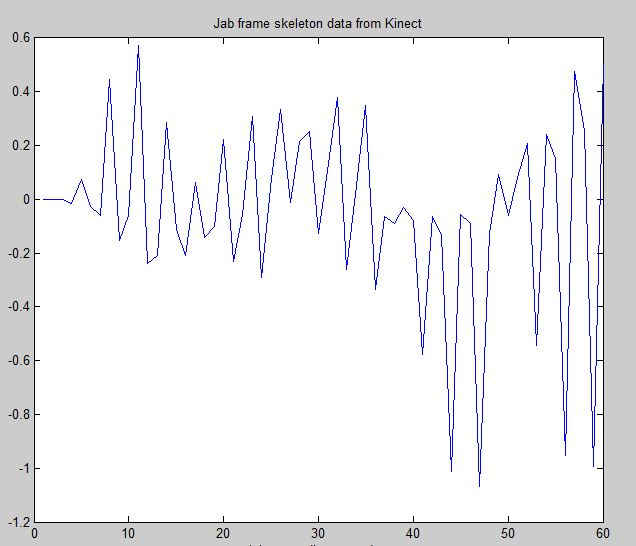
\includegraphics[height=0.10\textheight]{images/initjab}
    
    % \end{flushright}
    % \end{figure}

    % \begin{figure}[h]
    %     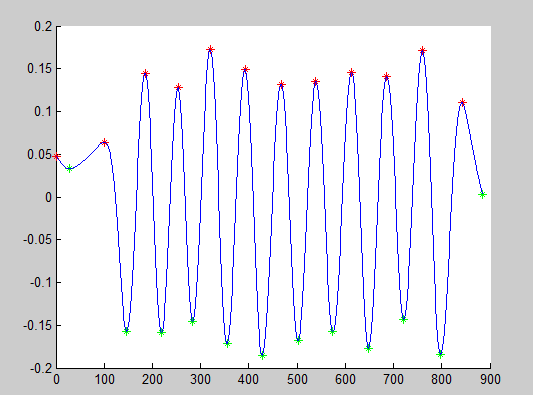
\includegraphics[height=0.10\textheight]{images/jabseg}
    %     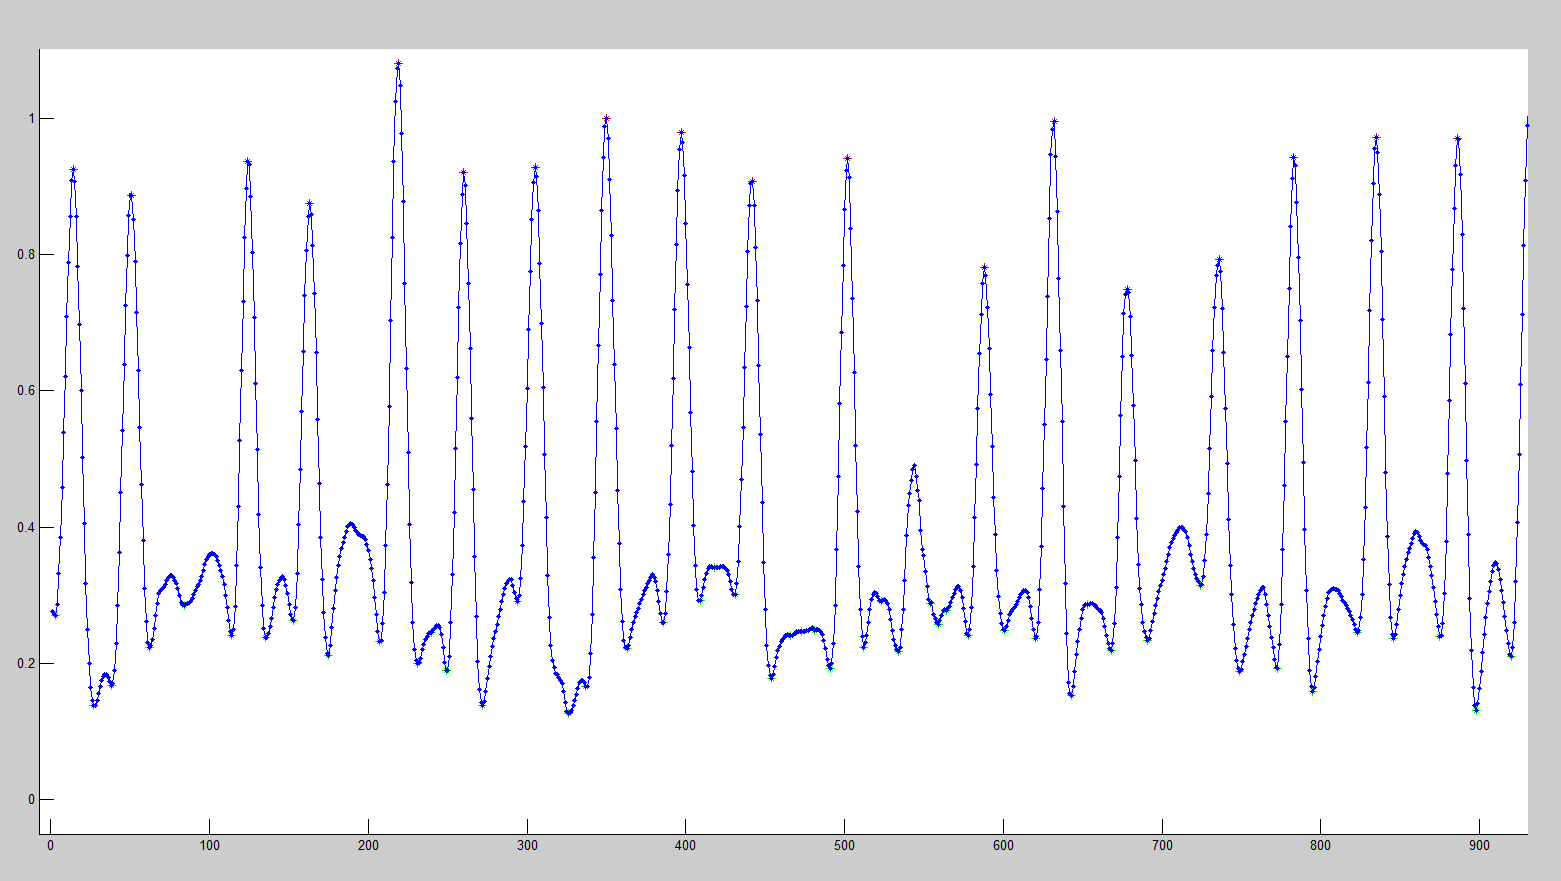
\includegraphics[height=0.10\textheight]{images/crossseg}
    % \end{figure}

    \begin{figure}[h]
        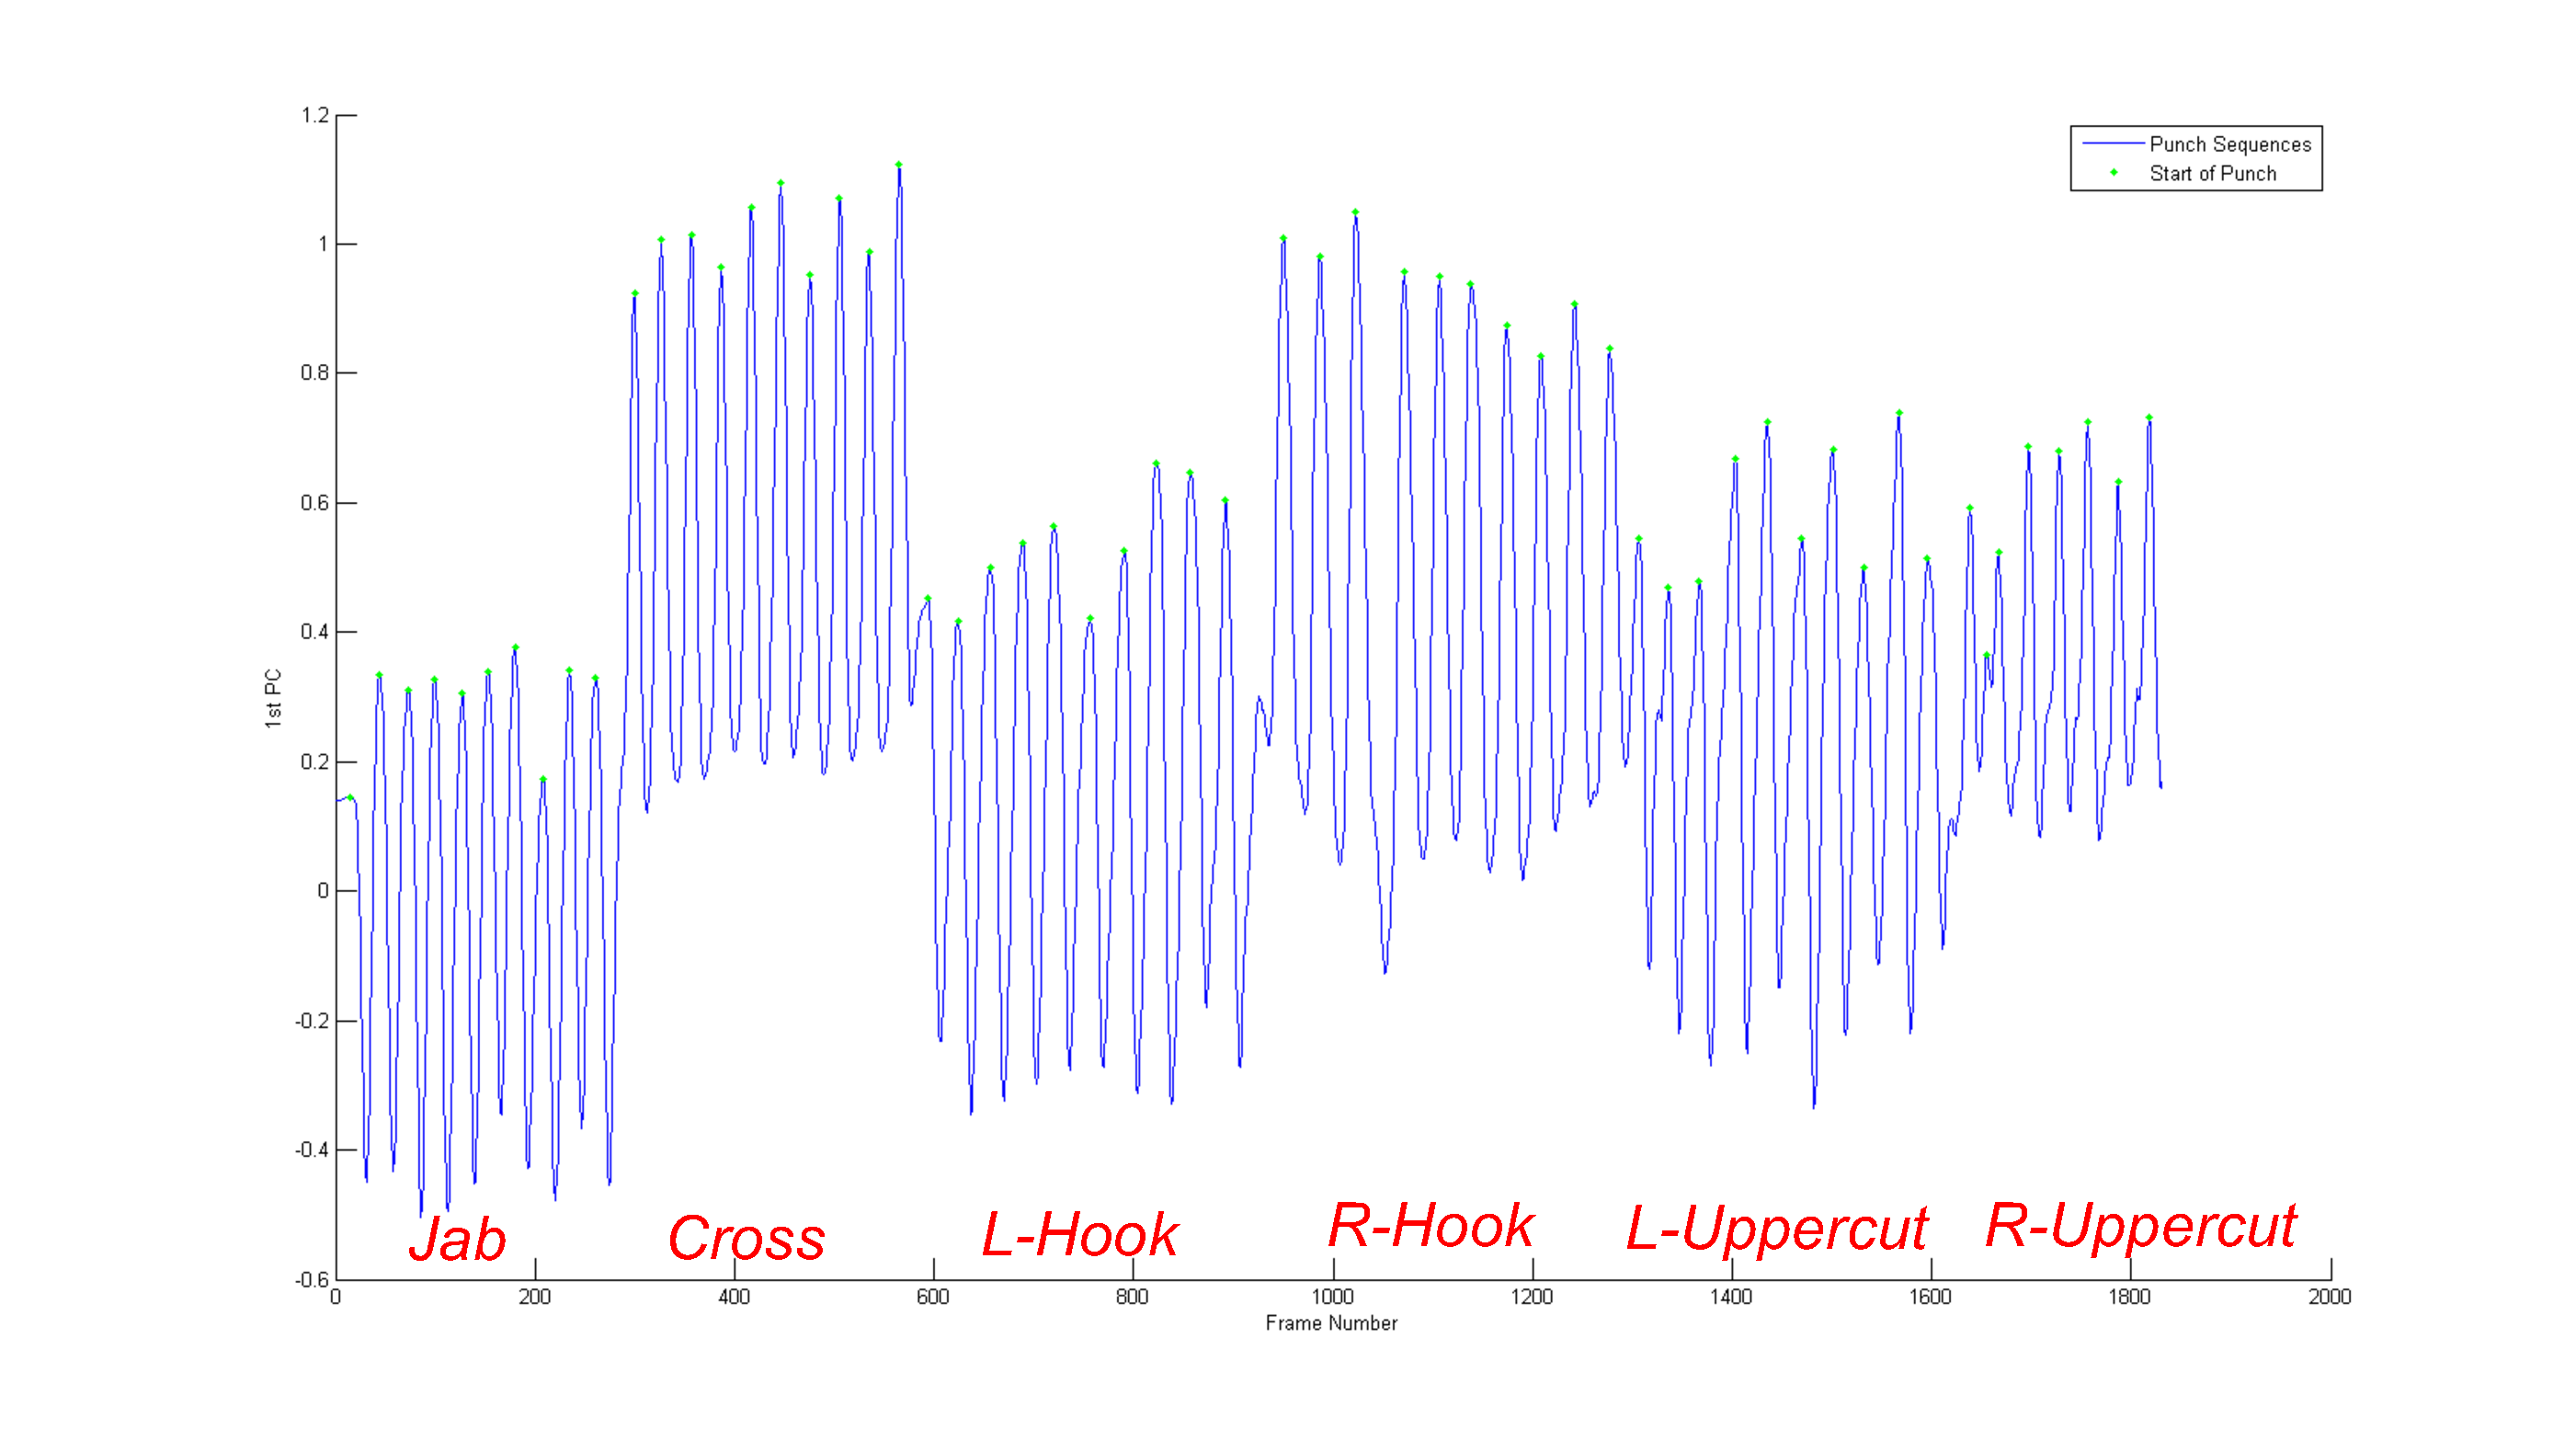
\includegraphics[height=0.15\textheight, width=0.35\textheight]{images/punchseq-pdf}
    \end{figure}
    The aim of the shout group is to minimise the amount of information that a hostile sender can gain about the peers' IP addresses. Here, we also need to consider the cases where members of the shout group are hostile and how we reduce the frequency of these attacks.
    \end{block}
    \end{column}
\end{columns}

%\vfill

\begin{columns}[t]
    \begin{column}{0.422\linewidth}
    \begin{block}{\normalsize 3. Classification}
    \small Peers are associated with a public key. This can reveal who is communicating with whom, even with anonymous identities. To prevent this I have invented a method of hiding a public key such that it becomes unrecognisable but so that it can still be used for encryption. In ElGamal, this can be done as follows:
    \begin{figure}[h]
        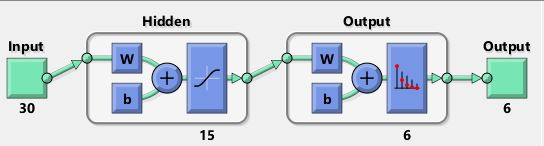
\includegraphics{images/neuralnet}
    \end{figure}    
    NOTE!
    \end{block}
    \end{column}
    
    \begin{column}{0.422\linewidth}
    \begin{block}{\normalsize 4. Results}
    \small The detection rate when classifying a sequence of mixed punches correctly goes from $85\%-93\%$. On a two-class problem such as good jabs and bad jabs a 99\% detection rate has been achieved.
    \begin{figure}[h]
        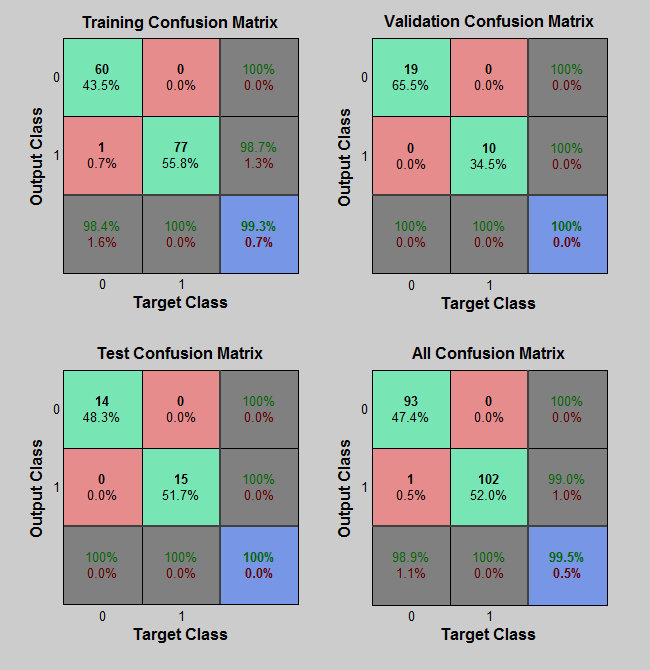
\includegraphics[height=0.15\textheight]{images/confm2}
        \vspace{1.00mm}
        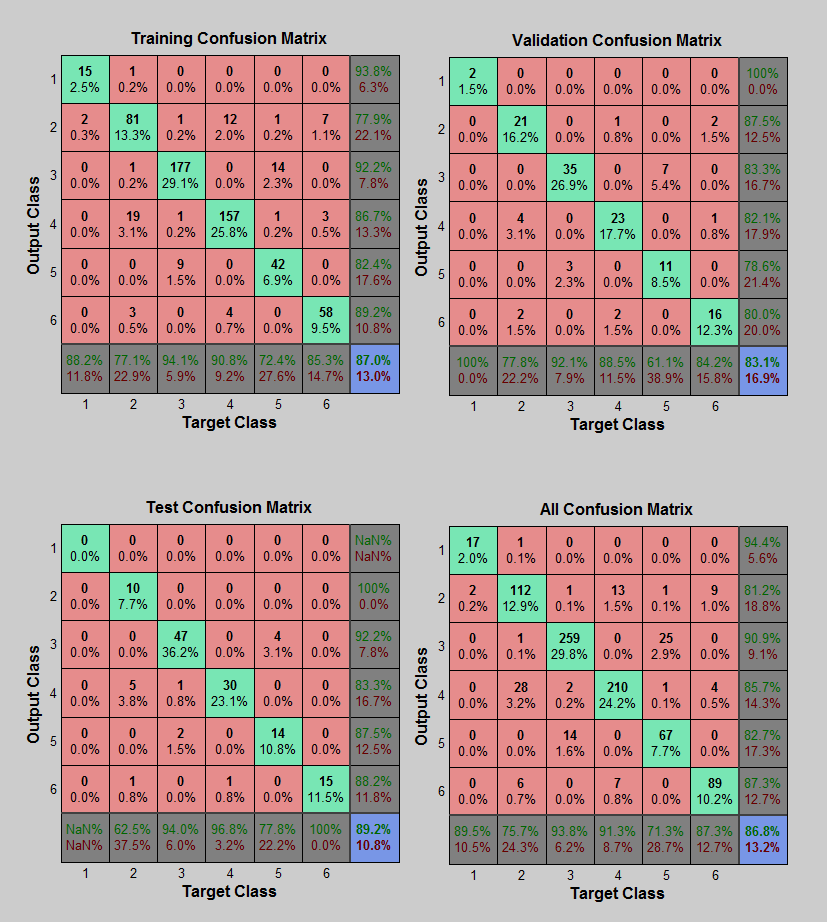
\includegraphics[height=0.15\textheight]{images/confm6}
    \end{figure}
    Nodes transform packets that pass through them so that packets cannot be traced. By using source routing, the sender can be assured that their packets are routed randomly.
    \end{block}
    \end{column}
\end{columns}

\vfill

\end{frame}

% -----------------------------------------------------------------------------

\end{document}



